Veamos la siguiente figura

\begin{figure}[ht!]
    \centering
    \begin{tikzpicture}[auto, node distance=1.5cm]
        % Estilos de los elementos
        \tikzset{
            block/.style = {draw, fill=blue!8, rectangle, minimum height=2.8em, minimum width=4.5em, rounded corners=2pt},
            sum/.style   = {draw, fill=white, circle, minimum size=6mm},
            coord/.style = {coordinate}
        }

        % Nodos de bloques
        \node [coord] (input) {};
        \node [sum, right=1.2cm of input] (sum) {};
        \node [block, right=1.5cm of sum] (plant) {Sistema $G(s)$};
        \node [coord, right=1.2cm of plant] (branch) {};
        \node [coord, right=1.2cm of branch] (output) {};
        \node [block, below=1.0cm of plant] (sensor) {Compensador $H(s)$};

        % Flujo directo (Camino directo)
        \draw [-Latex] (input) -- node {$R(s)$} (sum);
        \draw [-Latex] (sum) -- node {$E(s)$} (plant);
        \draw [-Latex] (plant) -- (branch);
        \draw [-Latex] (branch) -- node {$Y(s)$} (output);

        % Bucle de retroalimentación
        \draw [-Latex] (branch) |- (sensor);
        \draw [-Latex] (sensor) -| (sum);

        % Signos de la suma/resta
        \node at ($(sum.west) + (0.15, 0)$) {\small $+$};
        \node at ($(sum.south) + (0, 0.15)$) {\small $-$};

        % Punto de ramificación
        \fill (branch) circle (1.5pt);

    \end{tikzpicture}
    \caption{Diagrama de bloques de un sistema de control retroalimentado sin controlador.}
    \label{fig:sistema_control_retroalimentado}
\end{figure}


\noindent Dicha figura representa un sistema de control retroalimentado mediante $H(s)$. En la salida del punto suma se representa el error que surge entre la entrada y la salida multiplicada por el compensador. El error es entonces

\begin{equation*}
    E(s) = R(s) - H(s)Y(s)
\end{equation*}

\noindent Si dividimos el error por la entrada, se obtiene

\begin{equation*}
    \frac{E(s)}{R(s)} = 1 - \frac{H(s)Y(s)}{R(s)} 
\end{equation*}


\noindent Pero $Y(s)/R(s)$ es la función de transferencia en lazo cerrado, por lo tanto

\begin{equation*}
    \frac{E(s)}{R(s)} = 1 - H(s)\left(\frac{G(s)}{1+H(s)G(s)}\right) = \frac{1}{1 + G(s)H(s)}
\end{equation*}


El teorema del valor final ofrece una forma conveniente de determinar el comportamiento en estado estacionario de un sistema estable. Como $E(s)$ es 


\begin{equation*}
    E(s) = \frac{1}{1 + G(s)H(s)} R(s)
\end{equation*}


\noindent el error en estado estacionario es


\begin{equation}
    \label{eq:5}
    e_{ss} = \lim_{t\to\infty}e(t) = \lim_{s\to 0} sE(s) = \lim_{s \to 0} \frac{s}{1 + G(s)H(s)} R(s)
\end{equation}


La figura \ref{fig:2} representa el sistema, donde los parámetros son:

\begin{figure}[ht!]
    \centering
    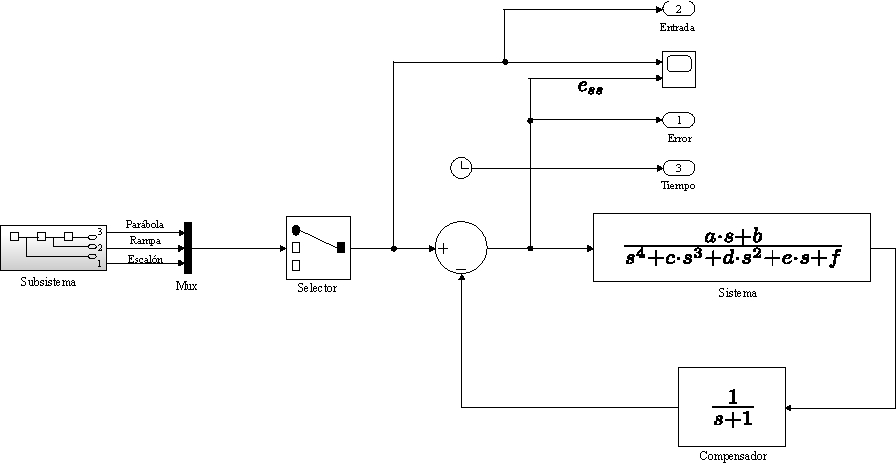
\includegraphics[width=0.8\textwidth]{imagenes/sistema.pdf}
    \caption{Sistema de control retroalimentado. El subsistema representa 3 entradas: escalón, rampa y parábola. Se utiliza un \textit{Selector} para elegir de forma dinámica el tipo de entrada que quiero recibir en el sistema.}
    \label{fig:2}
\end{figure}


\begin{equation*}
    a = 1, \qquad b = 2, \qquad c = 1, \qquad d = 10, \qquad e = 5, \qquad f = 8
\end{equation*}

La siguientes figuras representan el error para los 3 tipos de entradas establecidos anteriormente


\begin{figure}[ht!]
    \centering
    \begin{tikzpicture}
        \begin{groupplot}[
            group style={
                group size=2 by 2,
                horizontal sep=1.5cm,
                vertical sep=1.5cm
            },
            width=8cm,
            height=6.5cm,
            grid = both,
            xlabel = $t$
        ]
            % Gráfica 1 (Arriba Izquierda)
            \nextgroupplot[title=Escalón,
            legend entries = {$H(t)$, $e_p$},
            legend style = {at = {(0.95, 0.7)}, overlay}]
            \addplot[thick, domain = 0:20] {1};
            \addplot[thick, dashed] table [x = t, y = y]{archivos/escalon_error.txt};
            
            % Gráfica 2 (Arriba Derecha)
            \nextgroupplot[title=Rampa,
            legend entries = {$t$, $e_v$},
            legend pos = south east]
            \addplot[thick, domain = 0:20] {x};
            \addplot[thick, dashed] table [x = t, y = y]{archivos/rampa_error.txt};
            
            % Gráfica 3 (Abajo Centrada)
            % xshift = (6cm / 2) + (1.5cm / 2) = 3.75cm
            \nextgroupplot[
                title=Parábola,
                xshift=3.75cm,
                legend entries = {$1/2t^2$, $e_v$},
                legend pos = north west
                ]
            \addplot[thick, domain = 0:20] {0.5*x^2};
            \addplot[thick, dashed] table [x = t, y = y]{archivos/parabola_error.txt};
        \end{groupplot}
    \end{tikzpicture}
    \caption{Errores del sistema asociados a distintas entradas. Se observa que en cada una de ellas existe una diferencia entre la entrada y el error del sistema.}
    \label{fig:errores}
\end{figure}


Si evaluamos el límite \ref{eq:5} para una entrada escalón, obtenemos:

\begin{equation}
    e_{ss} = e_p = \frac{1}{\frac{b}{f} + 1} = \frac{f}{b + f} = \frac{4}{5} = 0.8
\end{equation}


\noindent el cual quiere decir que el error según entrada escalón es del $80\%$ (Observece la figura \ref{fig:errores} para la entrada escalón).

Ahora bien, cambiemos la retroalimentación (compensador) por la siguiente función transferencia: $1/s$. Ahora si evaluamos el límite para la entrada escalón, se obtiene el resultado de $0$, es decir que no hay error en la entrada escalón para el sistema. Ahora, si la entrada es una rampa 

\begin{equation}
    e_{ss} = e_v = \frac{f}{b} = 4
\end{equation}


\noindent Es decir, el error de velocidad es del $400\%$. A diferencia del compensador analizado previamente, el error velocidad divergía. 


\begin{figure}[ht!]
    \centering
    \begin{tikzpicture}
        \begin{groupplot}[
            group style={
                group size=2 by 1,
                horizontal sep=1.5cm,
                vertical sep=1.5cm
            },
            width=8cm,
            height=6.5cm,
            grid = both,
            xlabel = $t$
        ]
            % Gráfica 1 (Arriba Izquierda)
            \nextgroupplot[title=Escalón,
            legend entries = {$H(t)$, $e_p$},
            legend style = {at = {(0.95, 0.7)}, overlay}]
            \addplot[thick, domain = 0:40] {1};
            \addplot[thick, dashed] table [x = t, y = y]{archivos/escalon_error_integrador.txt};
            
            % Gráfica 2 (Arriba Derecha)
            \nextgroupplot[title=Rampa,
            legend entries = {$t$, $e_v$},
            legend pos = south east]
            \addplot[thick, domain = 0:5] {x};
            \addplot[thick, dashed] table [x = t, y = y]{archivos/rampa_error_integrador.txt};
        \end{groupplot}
    \end{tikzpicture}
    \caption{Errores del sistema asociados a distintas entradas pero con un integrador como compensador. Para la entrada escalón el error tiende a 0 pero para la entrada rampa el error converge a un límite (anteriormente divergía). Para la entrada parabólica sucede parecido al caso analizado anteriormente}
    \label{fig:errores2}
\end{figure}





Veamos el último caso: $H(s) = 1/s^2$. Para comprender qué pasa en este caso, podemos acudir a las funciones \texttt{tf}, \texttt{feedback} y \texttt{pole}. El siguiente código representa el cálculo de los polos para el sistema.



\begin{lstlisting}[caption = {Cálculo de los polos al sistema}, label = {cod:3}]
a = 1;
b = 2;
c = 1;
d = 10;
e = 5;
f = 8;

Gs = tf([a, b], [1, c, d, e, f]);
Hs = [tf([1], [1, 1]), tf([1], [1, 0]), tf([1], [1, 0, 0])];
Fs = feedback(Gs, Hs(3)); %función transferencia de lazo cerrado
polos_fs = pole(Fs);
\end{lstlisting}


Por lo tanto, para el sistema con compensador $1/s^2$ se obtienen los siguientes polos.


\begin{align*}
    &p_{1, 2} = -0.2484 \pm 2.9696 i\\
    &p_{3, 4} = -0.3506 \pm 0.7433 i\\
    &p_{5, 6} = 0.0991 \pm 0.5689 i
\end{align*}


\noindent Es decir, los polos presentan parte real positiva y por lo tanto el sistema es inestable.